\section{Summarizing Data}

\subsection{Methods Based on CDF}

\begin{definition}{\textbf{(Empirical CDF)}}
    Suppose we have $x_1,\dots,x_n$ be a batch of numbers. The empirical cumulative distribution function is defined as:
    \begin{equation*}
        F_n(x) = \frac{1}{n}(\# x_i \le x)
    \end{equation*}
    Or, we have an ordered number of $x_{(1)}\le x_{(2)} \le \cdots \le x_{(n)}$. We have: if $x_{(k)} \le x < x_{(k+1)}$, then $F_n(x) = k/n$. 
\end{definition}

\begin{remark}{\textbf{(Comments on Empirical CDF)}}
    In the analysis, it is better to express $F_n$ in the following way, given random variables $X_1,\dots,X_n$:
    \begin{equation*}
        F_n(x) = \frac{1}{n} \sum^n_{i=1} I_{(-\infty, x]}(X_i) \qquad \text{ where } \qquad I_{(-\infty, x]}(X_i) = \begin{cases}
            1 & \text{ if } X_i \le x \\
            0 & \text{ otherwise }
        \end{cases}
    \end{equation*}
    The random variable $I_{(-\infty, x]}(X_i)$ are independent Bernoulli random variables, where we have:
    \begin{equation*}
        I_{(-\infty, x]}(X_i) = \begin{cases}
            1 & \text{ with probability } F(x) \\
            0 & \text{ with probability } 1-F(x) \\
        \end{cases}
    \end{equation*}
    Thus, $nF_n(x)$ is a binomial random variable ($n$ trials with probability of $F(x)$ of success), as we have:
    \begin{equation*}
        \mathbb{E}[F_n(x)] = F(x) \qquad \operatorname{var}(F_n(x)) = \frac{1}{n}F(x)[1-F(x)]
    \end{equation*}
    An estimate of $F_n(x)$ is unbiased and has a maximum variacne at the value of $x$ such that $F(x) = 0.5$, which is at median. 
\end{remark}

\begin{remark}{\textbf{(Behavior of $\boldsymbol F_n$)}}
    If we consider the stochastic behavior of $F(x)$, then we can show that:
    \begin{equation*}
        \max_{-\infty<x<\infty} \abs{F_n(x) - F(x)}
    \end{equation*}
    doesns't depend on $F$ if $F$ is continuous. This allow us to construct a simultaneous confidence band about $F_n$, which can be used to test goodness-of-fit. Please note that this isn't the same compared to the confidence interval of binomial distribution. 
\end{remark}

\begin{definition}{\textbf{(Survival Function)}}
    It is equivalent to CDF and is defined as:
    \begin{equation*}
        S(t) = \mathbb{P}(T > t) = 1-F(t)
    \end{equation*}
    where $T$ is a random variable with CDF of $F$. We use it where the data consists of times until failure or death and so non-negative. $S(t)$ denotes the lifetime will be longer than $t$, and so we can have empirical version to be $S_n(t) = 1-F_n(t)$. 
\end{definition}

\begin{definition}{\textbf{(Hazard Function)}}
    It is interpreted as the instantaneous death rate for individual who have survived up to a given time. If an individual is alive at time $t$, the probability that the individual will die at time interval $(t, t + \delta)$ is (assuming density function $f$ is continuous at $t$):
    \begin{equation*}
    \begin{aligned}
        P(t \le T \le t + \delta | T\ge t) &= \frac{P(t\le T \le t + \delta)}{P(T \ge t)} \\
        &= \frac{F(t + \delta) - F(t)}{1 - F(t)} \approx \frac{\delta f(t)}{1-F(t)}
    \end{aligned}
    \end{equation*}
    The hazard function is defined as:
    \begin{equation*}
        h(t) = \frac{f(t)}{1-F(t)}
    \end{equation*}
    If $T$ is the lifetime of a manufactured component, it may be natural to think of $h(t)$ as the instantaneous or age-specific failure rate. 
\end{definition}

\begin{remark}{\textbf{(Interpretation of Hazard Function)}}
    It can be expressed as:
    \begin{equation*}
        h(t) = -\frac{d}{dt}\log[1-F(t)] = -\frac{d}{dt} \log S(t)
    \end{equation*}
    Which is the negative of the log of survival funcion. With the method of propagation of error:
    \begin{equation*}
        \operatorname{var}\Big( 1 - F_n(t) \Big) \approx \frac{\operatorname{var}[1-F_n(t)]}{(1-F(t))^2} = \frac{1}{n}\bracka{\frac{F(t)}{1-F(t)}}
    \end{equation*}
    For large value of $t$, the empirical log survial function is unrealiable, because $1-F(t)$ is very small, and so in practice, last few data are disregarded.
\end{remark}

\begin{remark}{\textbf{(Empirical Survial Function)}}    
    Suppose that there are no ties and the ordered failure times are: $T_{(1)} < T_{(2)} < \cdots < T_{(n)}$. If $t = T_{(i)}$, $F_n(t) = i/n$ and $S_{n}(t) = 1-i/n$. But since $\log S_n(t)$ is undefined for $t\ge T_{(n)}$, it is ofen defined as:
    \begin{equation*}
        S_n(t) = 1 - \frac{i}{n+1}
    \end{equation*}
    for $T_{(i)} \le t < T_{(i+1)}$
\end{remark}

\begin{definition}{\textbf{(Quantile-Qunatile Plot)}}
    If $X$ is a continuous random variable with a strictly increasing distribution function $F$, the $p$-th quantile of the to be value of $x$ such that: $F(x) = p$ or $x_p = F^{-1}(p)$. In Q-Q plot, the quantile of one distribution is plotted against another. 
\end{definition}

\begin{remark}{\textbf{(Usage of Q-Q)}}
    Suppose we have $2$ distributions:
    \begin{itemize}
        \item $F$ is a model for observations of a control group. 
        \item $G$ is a model for observations of a group that has received some treatment. 
    \end{itemize}
    Let's consider how difference update changes the plot:
    \begin{itemize}
        \item Suppose that there is an effect changned by $h$ uniformly i.e $y_p = x_p + h$, where $y_p$ is the group that received the treatment and vice versa. This gives us the relationship to be: $G(y) = F(y - h)$. 
        \item Similarly, we have the effect with multiplicative differences i.e given $c \in \mathbb{R}$ where we have $y_p = cx_p$ with the relationship to be $G(y) = F(y/h)$
    \end{itemize}
    Given the number of samples, we have to use the empirical CDF to create thE Q-Q plot. Now, the results of the changes is shown in the following figure:
    \begin{figure}[H]
    \centering
    \begin{subfigure}{.5\textwidth}
        \centering
        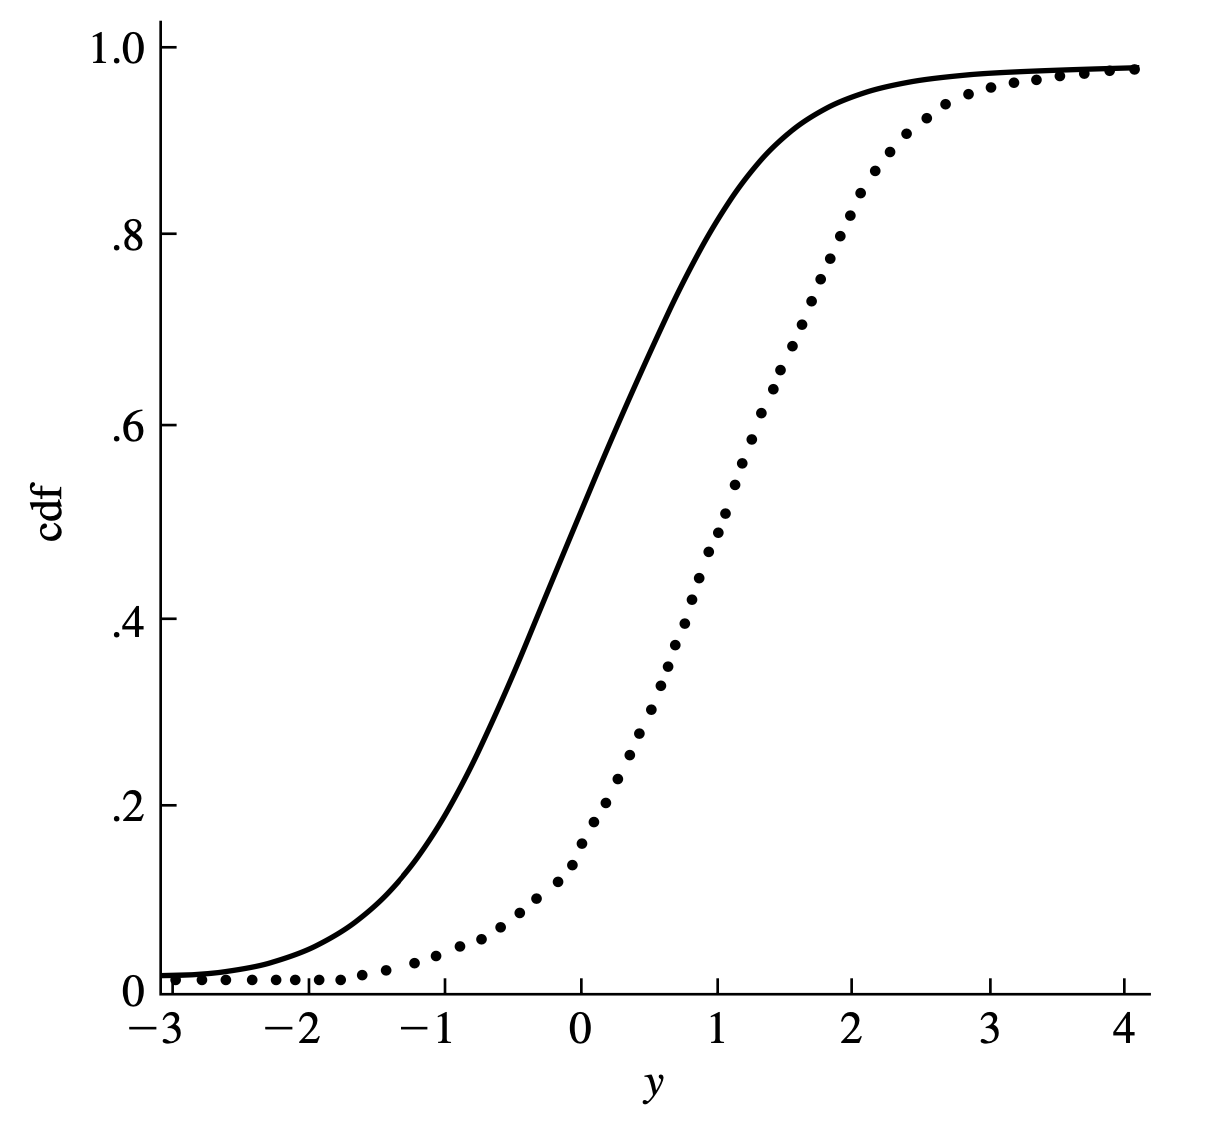
\includegraphics[width=0.7\linewidth]{img/img3.png}
        \caption{Additive Treatment Effect}
        \label{fig:1-sub1}
    \end{subfigure}%
    \begin{subfigure}{.5\textwidth}
        \centering
        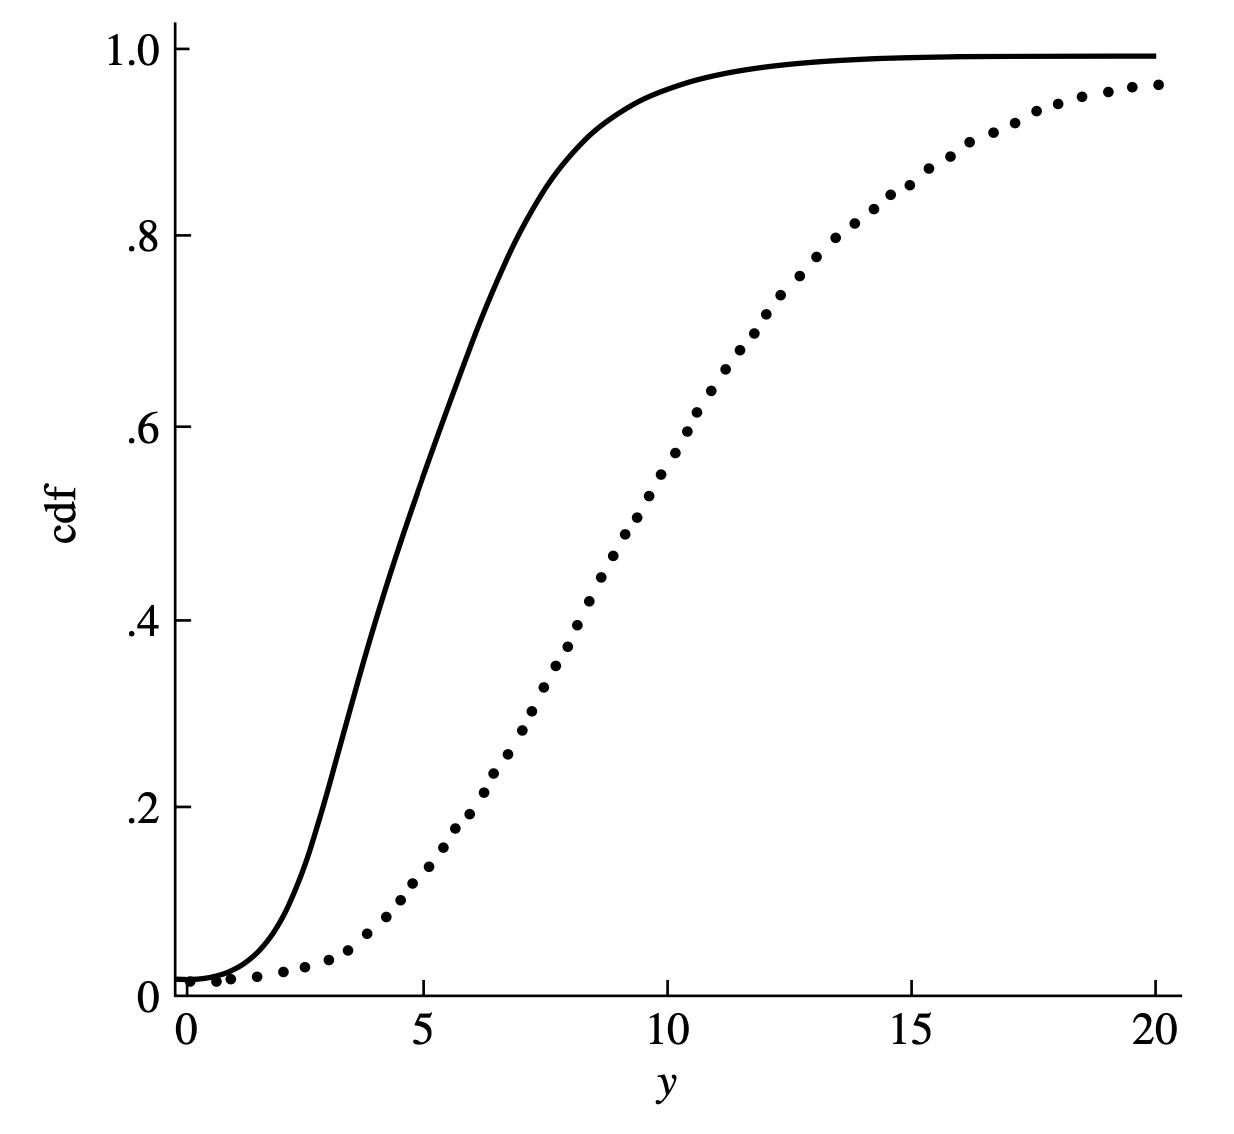
\includegraphics[width=0.7\linewidth]{img/img4.png}
        \caption{Multiplicative Treatment Effect}
        \label{fig:1-sub2}
    \end{subfigure}
    \end{figure}
\end{remark}

\begin{definition}{\textbf{(Kernel Probability Density Estimate)}}
    Let $w(x)$ be a non-negative, symmetric weight function, centered at zero and integrating to $1$. It can be standard normal density, with the following rescaled version:
    \begin{equation*}
        w_h(x) = \frac{1}{h}w\bracka{\frac{x}{h}}
    \end{equation*}
    is a rescaled version of $w$, as it approaches zero, $w_h$ becomes more concentrated and peaked around zero. On the other hand, as $h$ approaches infinity, $w_h$ becomes flat. If $X_1,\dots,X_n$ is a sample from a probability density function $p$, its esitmate is:
    \begin{equation*}
        f_h(x) = \frac{1}{n}\sum^n_{i=1}w_h(x - X_i)
    \end{equation*}
    The parameter $h$ represents bandwidth of estimating function as it controls the smoothness.
\end{definition}

\subsection{Meansure of Location}

\begin{definition}{\textbf{(Arithmetic Mean)}}
    The commonly used measure of location is the arithmetic mean, which is:
    \begin{equation*}
        \bar{x} = \frac{1}{n}\sum^n_{i=1}
    \end{equation*}
\end{definition}

\begin{remark}{\textbf{(Problem with Arithmeic Mean)}}
    By changing a single number, the arithmetic mean of a batch of numbers can be made arbitary large or smaller. Thus, when used blindly, without careful attention, the mean can produce a misleading results. Or, we need to have the measure of location that are robut or insensitive to outlier. 
\end{remark}

\begin{remark}{\textbf{(Why Sample Mean is Bad)}}
    The sample mean minimizers the log-likelihood of:
    \begin{equation*}
        \sum^n_{i=1}\bracka{\frac{(X_i - \mu)^2}{\sigma}}
    \end{equation*}
    This is the simpliest case of least square estimate. The outlier have a great effect on this estimate, as the deviation of $\mu$ from $X_i$ is measured by square of their difference.
\end{remark}

\begin{definition}{\textbf{(Median)}}
    It is a middle value of the ordered observation; if the sample size is even, the median is the average of the $2$ middle values. 
\end{definition}

\begin{proposition}{\textbf{(Confidence Interval)}}
    We can show that, given the population median $\eta$ and the interval between the order statistics $(X_{(k)}, X_{(n-k+1)})$
    \begin{equation*}
        P(X_{(k)} \le \eta \le X_{(n-k+1)}) = 1 - \frac{1}{2^{n-1}}\sum^{k-1}_{j=0}
    \end{equation*}
\end{proposition}
\begin{proof}
    The coverage probability of this interval is:
    \begin{equation*}
    \begin{aligned}
        P(X_{(k)} \le \eta \le X_{(n-k+1)}) &= 1 - P(\eta < X_{(k)} \text{ or } \eta > X_{n-k+1}) \\
        &= 1 - P(\eta < X_{(k)}) - P(\eta > X_{(n-k+1)})
    \end{aligned}
    \end{equation*}
    Since the event are mutually exclusive. To evaluate both terms, we note that:
    \begin{equation*}
    \begin{aligned}
        &P(\eta > X_{(n-k+1)}) = \sum^{k-1}_{j=0} \mathbb{P}(j \text{ observations} > \eta) \\
        &P(\eta < X_{(k)}) = \sum^{k-1}_{j=0} \mathbb{P}(j \text{ observations } < \eta)
    \end{aligned}
    \end{equation*}
    The median satisfies $P(X_i > \eta ) = P(X_i < \eta) = 1/2$, since $n$ observations $X_1,\dots,X_n$ are independent and identically distributed, the distribution of the number of observation greater than median is binomial with $n$ trials and probability $1/2$:
    \begin{equation*}
        P(j \text{ observations } > \eta) = \frac{1}{2}\begin{pmatrix}
            n \\ j
        \end{pmatrix}
    \end{equation*}
    and, so we have:
    \begin{equation*}
        P(\eta > X_{(n-k+1)}) = \frac{1}{2^n}\sum^{k-1}_{j=0}\begin{pmatrix}
            n \\ j
        \end{pmatrix}
    \end{equation*}
    This is the same for $P(\eta < X_{(k)})$ due to symmetry. Plugging it back to finish the proof
\end{proof}

\begin{remark}
    Median can be seen as the minimizer of the following loss:
    \begin{equation*}
        \sum^n_{i=1}\abs{\frac{X_i - \mu}{\sigma}}
    \end{equation*}
    Here, large deviation are not weighted as heavily, making median robust. The proof follows from the fact that the dervative of absolute is $\operatorname{sgn}(\cdot)$, and so the loss is zero when the positive $x - \mu$ (of the normalized data ) is equal to the negative item $x - \mu$, which is where the median situates. 
\end{remark}

\begin{definition}{\textbf{(Trimmed Mean)}}
    The $100\alpha\%$ trimmed mean consider the valuse that is between the lower $100\alpha\%$ and the higher $100\alpha\%$, as we can write it as:
    \begin{equation*}
        \bar{x}_\alpha = \frac{x_{[n\alpha] + 1} + \cdots + x_{(n - [n\alpha])}}{n - 2[n\alpha]}
    \end{equation*}
    where $[n\alpha]$ denotes the greatest integer less than or equal to $n\alpha$.
\end{definition}

\begin{definition}{\textbf{(M-Estimates)}}
    Consider the class of esitmates called $M$-estimates, where it is a minimizer:
    \begin{equation*}
        \sum^n_{i=1}\Psi\bracka{\frac{X_i - \nu}{\sigma}}
    \end{equation*}
    where $\Psi$ is the weight function that is a compromise between weight function for mean and median. 
\end{definition}

\begin{remark}{\textbf{(Measure of Dispersion)}}
    The most commonly used measure is sample standard deviation, where it is given as:
    \begin{equation*}
        S^2 = \frac{1}{n-1}\sum^n_{i=1}(X_i - \bar{X})^2
    \end{equation*}
    Using $n-1$ as divisor gives unbiased estimate. But like a sample mean standard deviation is sensitive to outlying observation. Two simple robust measures alternative are:
    \begin{itemize}
        \item Interquartile range (IQR): Differences between $2$ sample quantiles.
        \item Median absolute deviation from the median (MAD): If data are $x_1,\dots,x_n$ with median $\tilde{x}$, then MAD is the median of number $\abs{x_1,\dots,x_n}$. 
    \end{itemize}
\end{remark}


